\documentclass{article}

\title{Advanced Computer Graphics\\Exercise 2}
\author{Phil\'emon Favrod \and Solal Pirelli \and J\'er\'emy Rabasco}

\usepackage{amsmath}
\usepackage{tikz}
\usetikzlibrary{decorations.pathreplacing}
\usepackage{enumerate}

\begin{document}

\maketitle

\section*{Question 2.2.3}
In this answer, we will assume the following:
\begin{itemize}
\item Floating point numbers are actually considered as real numbers; and
\item \textit{drand48()} is a perfect uniform random generator in the interval $[0, 1]$.
\end{itemize}
The probability that the loop ends at a given iteration is the probability that a randomly selected point inside a cube with edges of length two is contained inside the upper hemisphere of the inscribed unit sphere. Therefore, it can be computed as
$$
\frac{V_{\text{Hemisphere}}}{V_{\text{Cube}}} = \frac{V_{\text{Sphere}}}{2V_{\text{Cube}}} = \frac{\frac{4}{3}\pi}{2^4} = \frac{\pi}{12} \approx 0.2618. 
$$

We are now wondering the expected value of a random variable following a Geometric distribution with probability of success being $p = \frac{\pi}{12}$. Therefore,
the expected number of iterations is $\frac 1p = \frac{12}{\pi} \approx 3.8197$.

\section*{Question 2.3.1}
The challenge here is to find a uniformly distributed point of the unit hemisphere given two random rel numbers uniformly distributed between 0 and 1, say $\xi_1$ and $\xi_2$. The reader might refer to Figure \ref{fig:hemisphere} to understand our solution. It basically proceeds as follows:
\begin{enumerate}[1.]
\item A rand point $r$ uniformly distributed over the circular surface which is the base of our hemisphere is generated. The methods presented in class is used here, i.e. $(\sqrt{\xi_1}, 2\pi\xi_2)$ is used instead of the naive but biased approach that takes $(\xi_2, 2\pi\xi_2)$ as a random point\footnote{The points of this sentence are represented in polar coordinates in the XY plane.}. As a reminder, the problem with the later is that points near the center of the circular surface are more likely to be picked. 
\item Then, this random point is projected onto the hemisphere surface by a simple application of the Pythagorean theorem resulting, in a Cartesian coordinate system, in the point
$$
p = (\sqrt{\xi_1}\cos{\left( 2\pi\xi_2\right)}, \sqrt{\xi_1}\sin{\left( 2\pi\xi_2\right)}, \sqrt{1 - \xi_1}).
$$
\end{enumerate}




\begin{figure}[h]
\centering
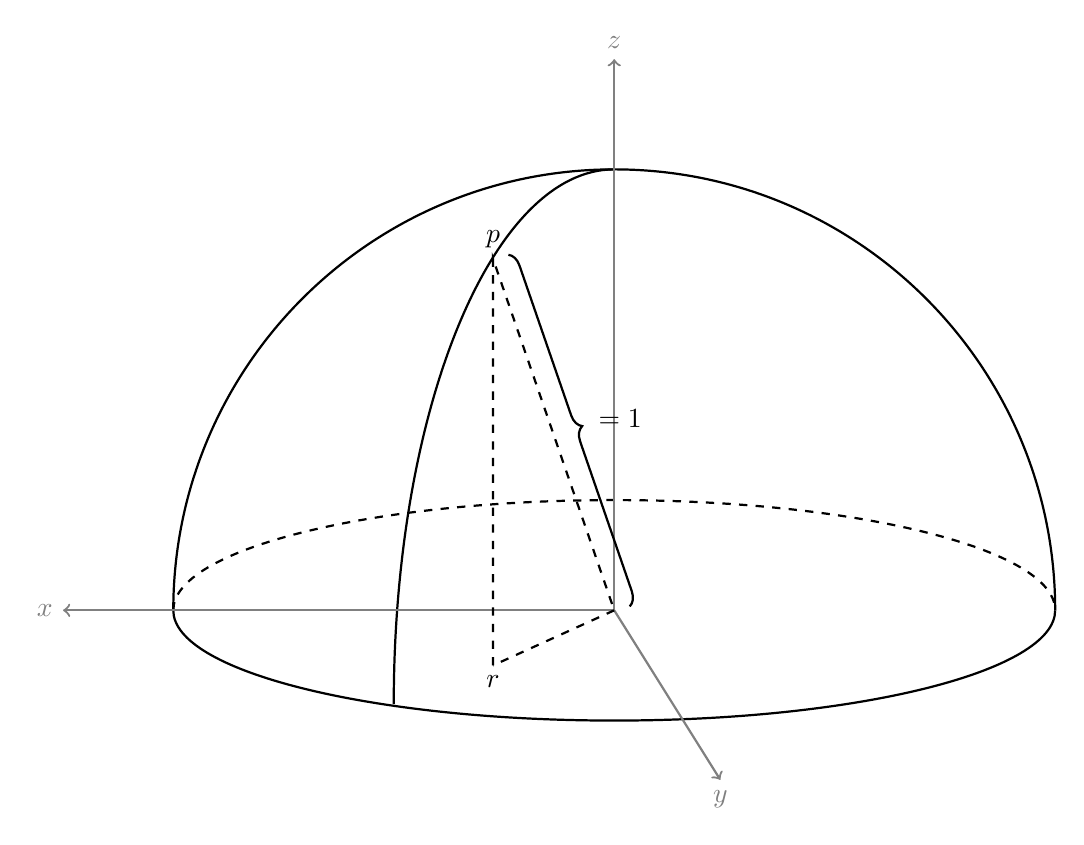
\begin{tikzpicture}[thick, scale=1.4]
% base circle
\draw (0,0) arc (180:360:4 and 1);
\draw [dashed] (0,0) arc (180:0:4 and 1);

% hemisphere
\draw (0,0) arc (180:0:4 and 4);
\draw (2,-.85) arc (180:90:2 and 4.85);

% axes
\draw [->, gray] (4,0,0) -- ++(-5,0,0)node[anchor=east]{$x$};
\draw [->, gray] (4,0,0) -- ++(0,-2.5,-2.5)node[anchor=north]{$y$};
\draw [<-, gray] (4,5)node[anchor=south]{$z$} -- (4, 0);

% schema
\draw [dashed] (4,0) -- (2.9,-0.5)node[anchor=north] {$r$};
\draw [dashed] (2.9, -0.5) -- (2.9, 3.19)node[anchor=south] {$p$} -- (4,0);
\draw [decorate,decoration={brace,amplitude=5pt},xshift=4pt,yshift=1pt]
(2.9, 3.19) -- (4,0) node [black,midway,xshift=0.65cm, yshift=0.15cm]{$= 1$};
\end{tikzpicture}
\caption{Generating a uniformly distributed random point of a unit hemisphere given two uniformly distributed random real numbers between 0 and 1.}
\label{fig:hemisphere}
\end{figure}

\section*{Question 3.3.2}
In this part, we want to estimate
$$
L_o(x, \omega_o) = \int_{H^2}f(x, \omega_i, \omega_o)L_i(x, \omega_i)(n \cdot \omega_i)d\omega_i
$$
where $L_o(x, \omega_o)$ represents the radiance reflected when an incoming ray $\omega_i$ with radiance $L_i(x, \omega_i)$ hits a point $x$ of a surface with normal $\hat n$. $\omega_i$, $\omega_o$ and $n$ are unit vectors in the above expression.

The Phong model provides us with the following BRDF:
$$
f(x, \omega_i, \omega_o) = f_d(x, \omega_i, \omega_o) + f_s(x, \omega_i, \omega_o) = \frac{k_d}{\pi} + k_s\frac{n + 2}{2\pi}(\omega_i \cdot s)^n
$$
where $s$ is a vector pointing in the perfect specular direction with respect to $\omega_o$.

We are trying to perform a backward ray-tracing with importance sampling, i.e. trying to guess the most important $\omega_i$ given $\omega_o$ and $x$ to determine $L_o(x, \omega_o)$. We therefore want to find the probability distribution function $p(\omega_i)$ such that the Monte Carlo estimator
$$F_N = \frac{1}{N}\sum\limits_{i=1}^N\frac{f(x, \omega_i, \omega_o)L_i(x, \omega_i)(n \cdot \omega_i)}{p(\omega_i)}
$$
is unbiased and has a small variance. The ideal case -- in which the estimator would actually be equal to the integral -- would be to choose a PDF proportional $f(x, \omega_i, \omega_o)L_i(x, \omega_i)(n \cdot \omega_i)$ but we don't know $\omega_i$ and therefore do not know $L_i(x, \omega_i)$. We therefore take the trade-off to choose $p(\omega_i)$ such that it is proportional to only $f(x, \omega_i, \omega_o)(n \cdot \omega_i)$.

\paragraph{Question 2.3.2a}
We chose $p(\omega_i)$ according to the provided paper. In this paragraph, we will try to capture the intuition out of these formulas. For simplicity reasons, it is easier to decompose $p(\omega_i)$ in its specular and diffuse component and choose $p_s(\omega_i)$ proportional to the specular component and $p_d(\omega_i)$ proportional to the diffuse component.

Regarding the diffuse component, the paper advises use to take $p_s(\omega_i) = \frac{n+1}{2\pi}\cos^n(\alpha)$ to get a ray distributed mainly near the specular direction.
One could be surprised that $\frac{n+2}{2\pi}(\omega_i \cdot s)^n(n \cdot \omega_i)$ was not simply chosen.
According to \cite{Lafortune}, the main reason is that it lacks integrability and so fails to be a PDF.

For the diffuse case, $p_d(\omega_i) = \frac{\cos(\theta_i)}{\pi}$ is the obvious choice. It favors ray that are evenly distributed ray around the surface normal at the point of intersection while limiting the numbers of sample with a 90 degree angle with the surface normal (those rays have little irradiance). 

Then with probability $\frac{k_s}{k_s + k_d}$ we chose a specular sampleand with probability $\frac{k_d}{k_s + k_d}$ we chose a diffuse sample. Thus, we perform multiple importance sampling with a schema that resembles balance heuristic to obtain

$$p(\omega_i) = \frac{k_s \cdot p_s(\omega_i) + k_d \cdot p_d(\omega_i)}{k_s + k_d}.$$

It is easy to see that this gives an unbiased estimator as the weights in the weighed average used to compute $p(\omega_i)$ are equal to the probabilities to choose a specular sample or a diffuse sample.

\paragraph{Question 2.3.2b}Once we have picked $\omega_i$, one can easily compute\linebreak 
$\cos\alpha := \omega_i \cdot s$ where $\alpha$ is the angle between $s$ and $\omega_i$. First note that $$\cos \left (\angle(\omega_o, n)\right ) = \cos \left ( \angle(n,s) \right ) = \omega_o\cdot n.$$ Similarly, we have that
$$\cos\left(\angle (n, \omega_i)\right) = \cos\left(\angle(n,s) + \alpha\right) = \omega_i \cdot n.$$
It follows that $\cos^{-1}{\left(\omega_i \cdot n\right)} - \cos^{-1}{\left(\omega_o\cdot n\right)} = \alpha.$

\section*{Results}

\subsection*{Naive/Lambertian Model}

\begin{figure}[p]
\centering
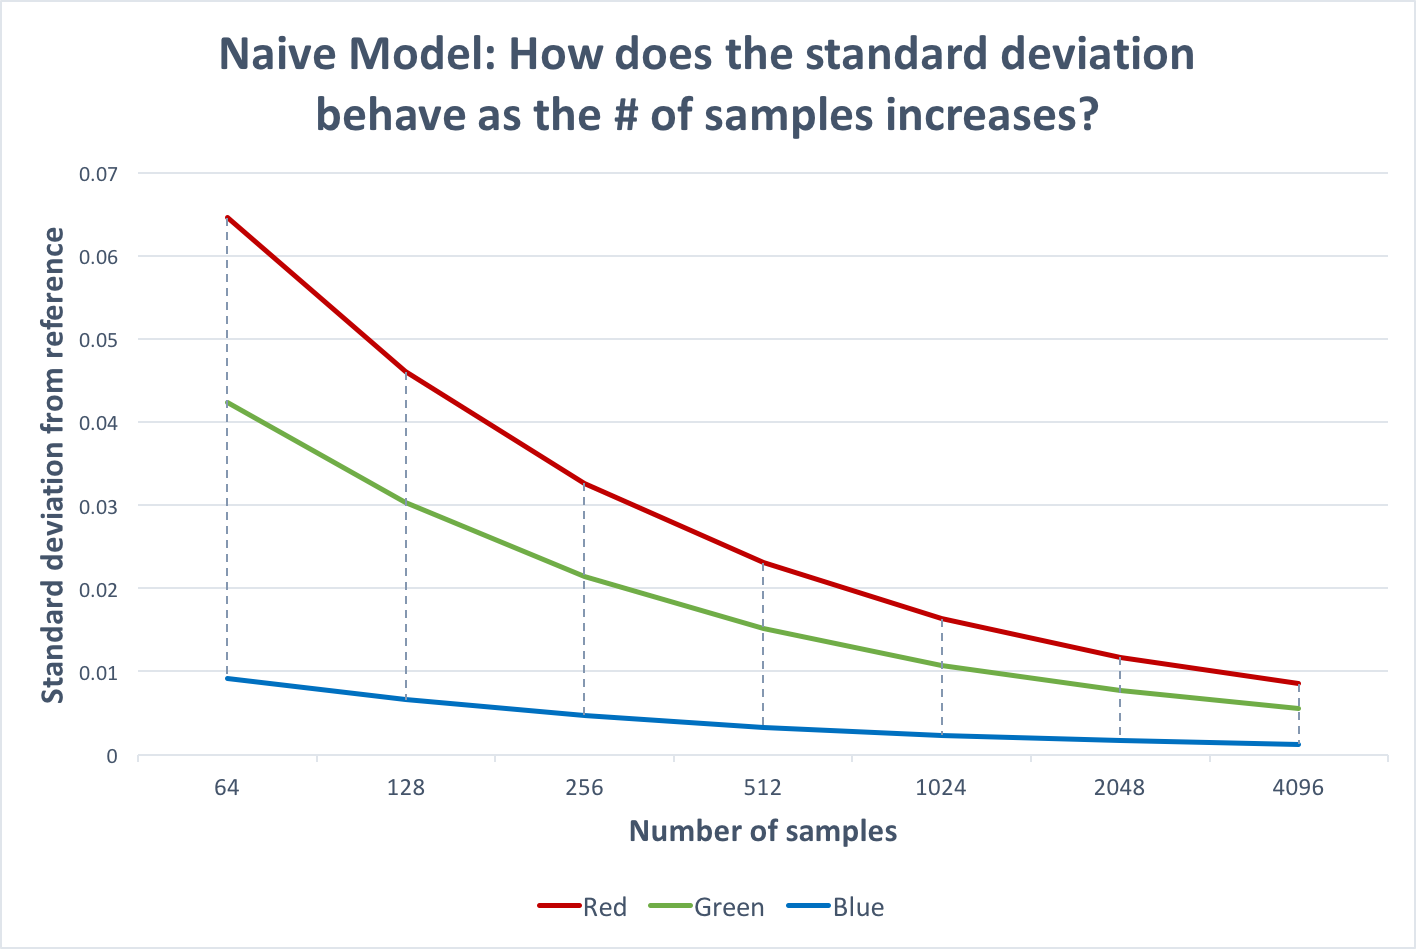
\includegraphics[width=\textwidth]{assets/naive_stdev}
\\
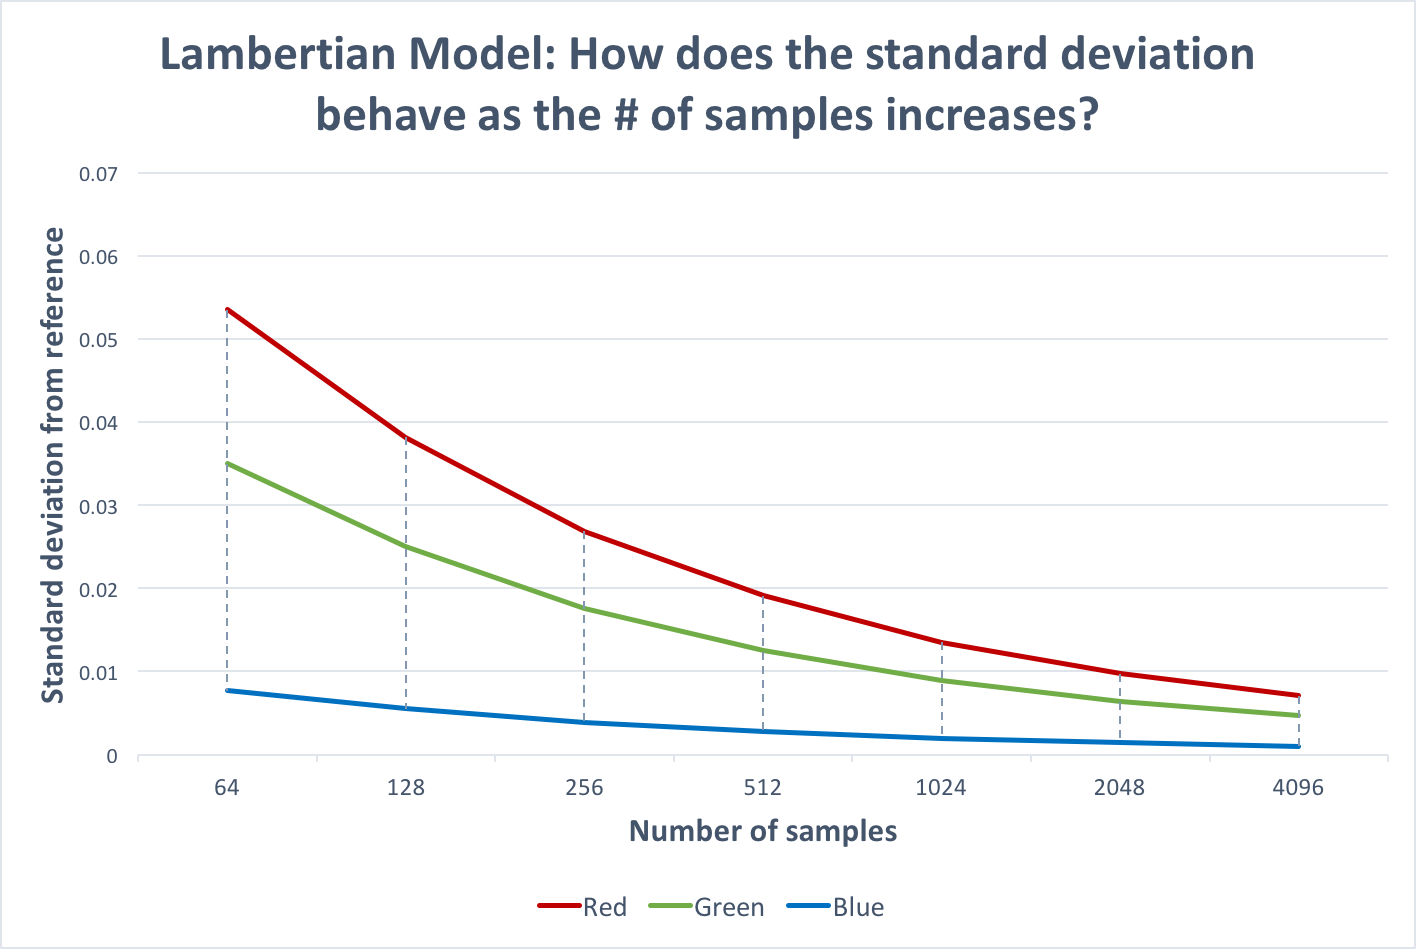
\includegraphics[width=\textwidth]{assets/lamb_stdev}

\caption{Comparison between the naive and the lambertian model convergence.}
\end{figure}


\clearpage
\subsection*{Phong Model}
\begin{figure}[h]
\centering
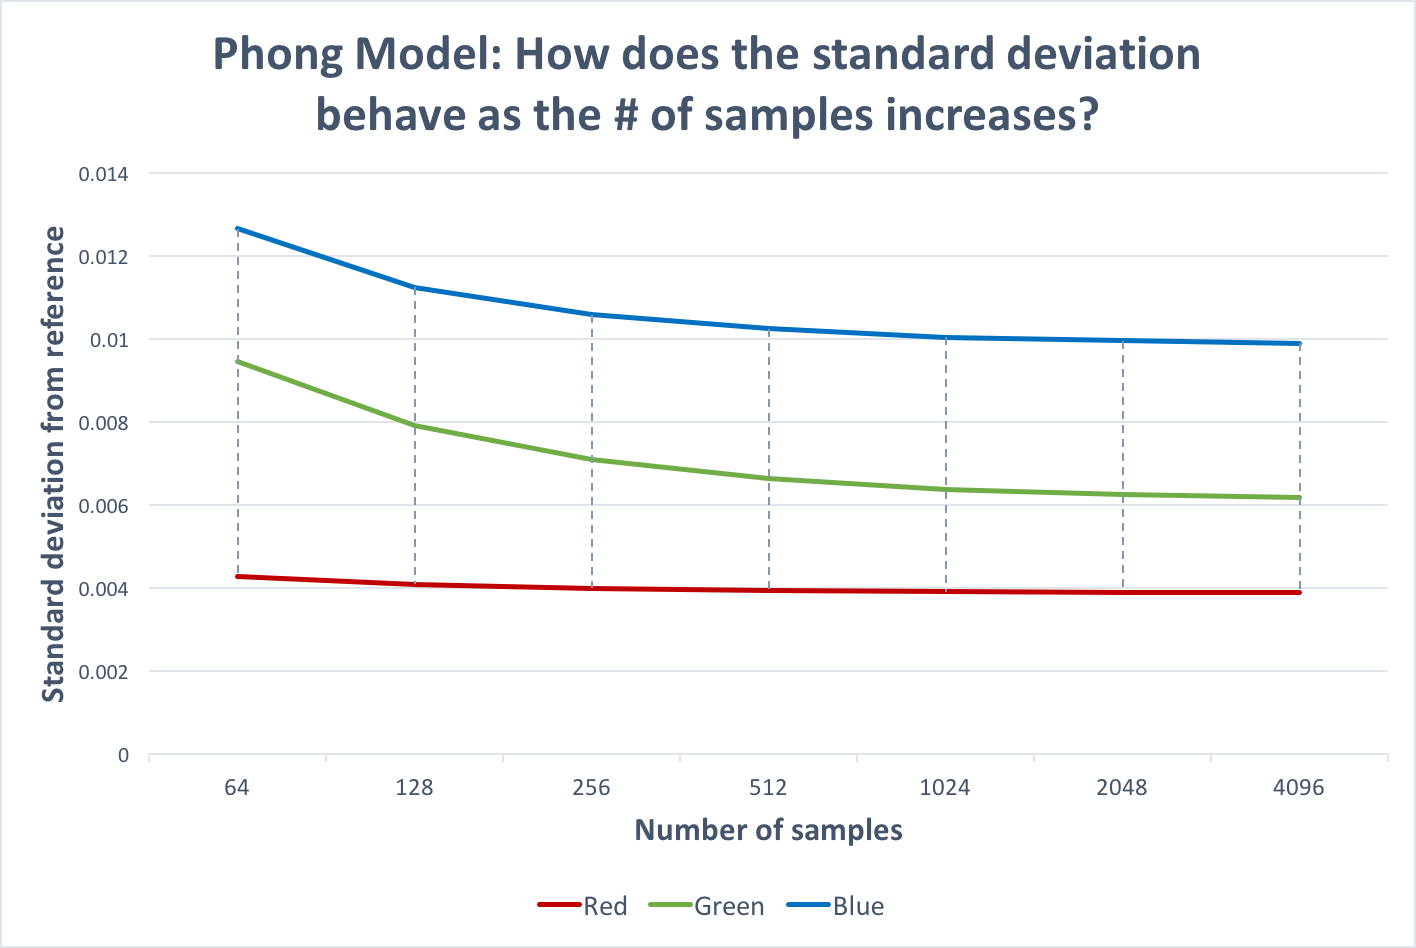
\includegraphics[width=\textwidth]{assets/phong_stdev}

\caption{Summary of the convergence of the Phong model.}
\end{figure}
\end{document}
